% Slides for the Lean 4 port of the EUTypes 2019 course
%   "Proving the correctness of a compiler" (Xavier Leroy).
%
% These slides are newly written for the Lean development in this repository.
% They follow the syllabus, section numbering and terminology of the original
% course, but contain no material copied from the original slide deck.
%
% Build with:  xelatex slides.tex   (twice, for the outline)

\documentclass[aspectratio=169,10pt]{beamer}

\usepackage{fontspec}
\usepackage{listings}
\usepackage{tikz}
\usepackage{amsmath,amssymb}
\usetikzlibrary{arrows.meta,positioning,calc}

\setmonofont{DejaVuSansMono.ttf}[
  Path=/usr/local/texlive/2021/texmf-dist/fonts/truetype/public/dejavu/,
  BoldFont=DejaVuSansMono-Bold.ttf,
  ItalicFont=DejaVuSansMono-Oblique.ttf,
  BoldItalicFont=DejaVuSansMono-BoldOblique.ttf,
  Scale=0.86]

\usetheme{default}
\usecolortheme{seagull}
\setbeamertemplate{navigation symbols}{}
\setbeamertemplate{itemize items}[circle]
\setbeamercolor{frametitle}{fg=black}
\setbeamerfont{frametitle}{series=\bfseries,size=\large}
\setbeamertemplate{frametitle}{%
  \vspace{2mm}\insertframetitle\par
  \vspace{-1mm}{\color{gray!60}\hrule height 0.4pt}\vspace{1mm}}
\setbeamertemplate{footline}{%
  \hfill{\tiny\color{gray}\insertframenumber\,/\,\inserttotalframenumber}\hspace{3mm}\vspace{2mm}}

\definecolor{kw}{RGB}{0,90,160}
\definecolor{cmt}{RGB}{110,110,110}
\definecolor{str}{RGB}{160,60,20}
\definecolor{hl}{RGB}{200,40,40}

\lstdefinelanguage{Lean}{
  morekeywords={theorem,def,abbrev,inductive,structure,instance,example,where,
    match,with,fun,let,have,show,from,by,intro,intros,exact,apply,refine,
    induction,cases,rcases,obtain,simp,omega,rfl,grind,namespace,end,open,
    import,variable,variables,deriving,termination_by,decreasing_by,mutual,
    partial,noncomputable,section,do,if,then,else,at,using,generalizing,
    calc,this,sorry,set_option,attribute},
  sensitive=true,
  morecomment=[l]{--},
  morecomment=[n]{/-}{-/},
  morestring=[b]",
}
\lstset{
  language=Lean,
  basicstyle=\ttfamily\small,
  keywordstyle=\color{kw}\bfseries,
  commentstyle=\color{cmt}\itshape,
  stringstyle=\color{str},
  showstringspaces=false,
  extendedchars=true,
  columns=fullflexible,
  keepspaces=true,
  aboveskip=1.2ex, belowskip=0.6ex,
  xleftmargin=1.5ex,
}
\newcommand{\code}[1]{\texttt{\small #1}}

\title{Proving the correctness of a compiler}
\subtitle{A Lean 4 development}
\author{Course material after Xavier Leroy, EUTypes 2019\\{\small Lean 4 port and slides}}
\date{}

\begin{document}

\begin{frame}[plain]
  \titlepage
  \begin{center}\small
  Slides written for the Lean~4 port in this repository.\\
  Original Coq course by Xavier Leroy, Collège de France and Inria Paris.
  \end{center}
\end{frame}

% ===================================================================
\section{Introduction}

\begin{frame}{Why prove a compiler correct?}
A compiler sits between the program you reasoned about and the program that
actually runs.
\medskip

\begin{itemize}
\item You verify the source. The machine runs the target.
\item Every guarantee you established --- by testing, by static analysis, by
      proof --- is only as good as the translation.
\item Compilers are not bug-free. Random-testing campaigns find miscompilations
      in every mainstream compiler.
\end{itemize}
\medskip

A miscompilation is especially nasty: the source is right, the reasoning is
right, and the bug is in the tool you trusted to be invisible.
\end{frame}

\begin{frame}{What would a theorem look like?}
Let $S$ be a source program and $C = \mathrm{compile}(S)$ its compiled form.
\medskip

\textbf{Semantic preservation}, informally:
\begin{center}
\emph{every observable behaviour of $C$ is an observable behaviour of $S$.}
\end{center}
\medskip

For our language the observable behaviours are:
\begin{itemize}
\item \emph{terminating} with a given final store,
\item \emph{diverging} (running forever),
\item \emph{going wrong} (getting stuck).
\end{itemize}
\medskip

We will prove: if $S$ terminates in store $s'$ then $C$ halts in $s'$;
and if $S$ diverges then $C$ diverges.  Compiled code never goes wrong.
\end{frame}

\begin{frame}{Two ingredients}
To even \emph{state} such a theorem we need formal semantics for both
languages.  To \emph{prove} it we need a proof assistant, because the case
analyses are large and unforgiving.
\medskip

This development uses \textbf{Lean 4}, with no library dependencies beyond
the core.
\medskip

Everything is machine-checked: no \code{sorry}, and the headline theorems
depend only on \code{propext}, \code{Classical.choice} and \code{Quot.sound}.
\end{frame}

\begin{frame}{Roadmap}
\begin{enumerate}\setlength{\itemsep}{2pt}
\item The source language: \textbf{IMP}
\item The target language: a \textbf{stack machine}
\item The \textbf{compilation scheme}
\item First correctness proofs --- terminating programs
\item[6.] Small-step semantics for IMP
\item[7.] Full correctness --- terminating \emph{and} diverging programs
\item[8.] An optimisation: \textbf{constant propagation}
\item[9.] More about \textbf{fixpoints}
\item[10.] \textbf{Liveness analysis} and dead code elimination
\end{enumerate}
\medskip
{\small (Section numbering follows the original course.)}
\end{frame}

% ===================================================================
\section{1. The source language: IMP}

\begin{frame}[fragile]{1.1 Arithmetic expressions}
\begin{lstlisting}
inductive aexp where
  | const (n : Int)
  | var   (x : Ident)
  | plus  (a₁ a₂ : aexp)
  | minus (a₁ a₂ : aexp)
\end{lstlisting}

A \emph{store} maps variables to their current values, and evaluation is an
ordinary recursive function --- a denotational semantics:

\begin{lstlisting}
def Store : Type := Ident → Int

def aeval (s : Store) : aexp → Int
  | .const n    => n
  | .var x      => s x
  | .plus  a₁ a₂ => aeval s a₁ + aeval s a₂
  | .minus a₁ a₂ => aeval s a₁ - aeval s a₂
\end{lstlisting}
\end{frame}

\begin{frame}[fragile]{What an evaluation function is good for}
\textbf{Run} a given expression in a given store:
\begin{lstlisting}
example : aeval (fun _ => 2)
    (.plus (.var "x") (.minus (.var "x") (.const 1))) = 3 := by native_decide
\end{lstlisting}

\textbf{Prove} a property of a given expression, for all stores:
\begin{lstlisting}
theorem aeval_xplus1 (s : Store) (x : Ident) :
    aeval s (.plus (.var x) (.const 1)) > aeval s (.var x)
\end{lstlisting}

\textbf{Prove a meta-property}, for all expressions at once --- the value of an
expression depends only on its free variables:
\begin{lstlisting}
theorem aeval_free {s₁ s₂ : Store} : ∀ a : aexp,
    (∀ x, freeInAexp x a → s₁ x = s₂ x) → aeval s₁ a = aeval s₂ a
\end{lstlisting}
This last kind is what compiler verification is made of.
\end{frame}

\begin{frame}[fragile]{1.3 Boolean expressions}
\begin{lstlisting}
inductive bexp where
  | true | false
  | equal     (a₁ a₂ : aexp)
  | lessequal (a₁ a₂ : aexp)
  | not (b₁ : bexp)
  | and (b₁ b₂ : bexp)
\end{lstlisting}

Everything else is a \emph{derived form} --- no new syntax, no new semantics
to prove sound:
\begin{lstlisting}
def bexp.greater (a₁ a₂ : aexp) : bexp := .not (.lessequal a₁ a₂)
def bexp.or (b₁ b₂ : bexp) : bexp := .not (.and (.not b₁) (.not b₂))

theorem beval_or (s : Store) (b₁ b₂ : bexp) :
    beval s (bexp.or b₁ b₂) = (beval s b₁ || beval s b₂)
\end{lstlisting}
\end{frame}

\begin{frame}[fragile]{1.4 Commands}
\begin{lstlisting}
inductive com where
  | skip
  | assign      (x : Ident) (a : aexp)
  | seq         (c₁ c₂ : com)
  | ifthenelse  (b : bexp) (c₁ c₂ : com)
  | while       (b : bexp) (c₁ : com)

infixr:80 " ;; " => com.seq
\end{lstlisting}

Euclidean division by repeated subtraction:
\begin{lstlisting}
def euclideanDivision : com :=
  .assign "r" (.var "a") ;;
  .assign "q" (.const 0) ;;
  .while (.lessequal (.var "b") (.var "r"))
    (.assign "r" (.minus (.var "r") (.var "b")) ;;
     .assign "q" (.plus (.var "q") (.const 1)))
\end{lstlisting}
\end{frame}

\begin{frame}[fragile]{The naive idea, and why it fails}
Why not an evaluation function for commands too?
\begin{lstlisting}
def cexec (s : Store) : com → Store
  | .skip       => s
  | .assign x a => update x (aeval s a) s
  | .seq c₁ c₂   => cexec (cexec s c₁) c₂
  | .while b c₁  => if beval s b then cexec (cexec s c₁) (.while b c₁) else s
\end{lstlisting}
\pause
Rejected --- rightly.  Every Lean function is total, but
\code{while true do skip} does not terminate.
\medskip

Worse: IMP is Turing-complete (unbounded loops, unbounded integers), so
\emph{no} computable function can return the final store when one exists and
report failure otherwise.
\end{frame}

\begin{frame}[fragile]{Big-step (natural) semantics}
Replace the function by a \emph{relation}: \code{cexec s c s'} holds exactly
when running \code{c} from \code{s} terminates in \code{s'}.
\begin{lstlisting}
inductive cexec : Store → com → Store → Prop where
  | skip   (s) : cexec s .skip s
  | assign (s x a) : cexec s (.assign x a) (update x (aeval s a) s)
  | seq : cexec s c₁ s' → cexec s' c₂ s'' → cexec s (c₁ ;; c₂) s''
  | ifthenelse : cexec s (if beval s b then c₁ else c₂) s' →
                 cexec s (.ifthenelse b c₁ c₂) s'
  | while_done : beval s b = false → cexec s (.while b c) s
  | while_loop : beval s b = true → cexec s c s' →
                 cexec s' (.while b c) s'' → cexec s (.while b c) s''
\end{lstlisting}
A derivation is a \emph{finite} tree.  Finiteness is exactly what rules out
non-terminating executions.
\end{frame}

\begin{frame}[fragile]{Divergence has no derivation}
\begin{lstlisting}
theorem cexec_infinite_loop (s : Store) :
    ¬ ∃ s', cexec s (.while .true .skip) s'
\end{lstlisting}
Proof: strengthen to ``no derivation concludes about
\code{while true do skip}'', then induct.  The \code{while\_done} case
contradicts \code{beval s .true = false}; the \code{while\_loop} case appeals
to the induction hypothesis.
\medskip
\pause

This is the strength \emph{and} the weakness of big-step semantics.

\begin{itemize}
\item Strength: termination is characterised precisely.
\item Weakness: divergence and going-wrong are both ``no derivation''.
      The semantics cannot tell them apart.
\end{itemize}
\medskip
We will need small-step semantics in \S6 for exactly this reason.
\end{frame}

\begin{frame}[fragile]{An interpreter, for testing}
The naive idea is salvageable if we bound the recursion depth:
\begin{lstlisting}
def cexecBounded : Nat → Store → com → Option Store
  | 0, _, _ => none
  | fuel + 1, s, c => match c with
    | .skip => some s
    | .seq c₁ c₂ => match cexecBounded fuel s c₁ with
        | none => none | some s' => cexecBounded fuel s' c₂
    | ...
\end{lstlisting}
Useless as a semantics, invaluable for trying programs out:
\begin{lstlisting}
example : (let s := update "a" 14 (update "b" 3 (fun _ => 0))
   (cexecBounded 100 s euclideanDivision).map (fun s' => (s' "q", s' "r")))
  = some (4, 2) := by native_decide
\end{lstlisting}
\end{frame}

% ===================================================================
\section{2. The target language}

\begin{frame}[fragile]{2.1 A stack machine}
Like an old RPN pocket calculator: a stack holds intermediate results;
each instruction pops its arguments and pushes its result.
\begin{lstlisting}
inductive instr where
  | const  (n : Int)        -- push n
  | var    (x : Ident)      -- push the value of x
  | setvar (x : Ident)      -- pop, assign to x
  | add                     -- pop two, push their sum
  | opp                     -- pop one, push its opposite
  | branch (d : Int)        -- skip d instructions
  | beq  (d₁ d₀ : Int)      -- pop two; skip d₁ if equal, d₀ if not
  | ble  (d₁ d₀ : Int)      -- pop two; skip d₁ if ≤, d₀ if >
  | halt                    -- stop

abbrev Code := List instr
\end{lstlisting}
Note: no subtraction instruction.  We will compile \code{a - b} as
\code{a + (-b)}.
\end{frame}

\begin{frame}[fragile]{2.2 Operational semantics}
A configuration is a program counter, a stack, and a store.  The code is
fixed throughout an execution.
\begin{lstlisting}
abbrev Config := Int × Stack × Store

def instrAt : Code → Int → Option instr
  | [], _        => none
  | i :: C', pc  => if pc = 0 then some i else instrAt C' (pc - 1)
\end{lstlisting}
Program counters are \emph{integers}, since branches may go backwards.
\begin{lstlisting}
inductive transition (C : Code) : Config → Config → Prop where
  | const : instrAt C pc = some (.const n) →
      transition C (pc, stk, s) (pc + 1, n :: stk, s)
  | branch : instrAt C pc = some (.branch d) → pc' = pc + 1 + d →
      transition C (pc, stk, s) (pc', stk, s)
  | ...
\end{lstlisting}
\end{frame}

\begin{frame}[fragile]{Three machine behaviours}
\code{halt} has \emph{no} transition --- that is what makes it stop the machine
rather than get it stuck.
\begin{lstlisting}
def machineTerminates (C) (sInit sFinal : Store) : Prop :=
  ∃ pc, transitions C (0, [], sInit) (pc, [], sFinal)
      ∧ instrAt C pc = some .halt

def machineDiverges (C) (sInit : Store) : Prop :=
  Infseq (transition C) (0, [], sInit)

def machineGoesWrong (C) (sInit : Store) : Prop :=
  ∃ pc stk s, transitions C (0, [], sInit) (pc, stk, s)
    ∧ Irred (transition C) (pc, stk, s)
    ∧ (instrAt C pc ≠ some .halt ∨ stk ≠ [])
\end{lstlisting}
Execution starts at \code{pc = 0} with an empty stack and succeeds when it
reaches a \code{halt} with an empty stack.
\end{frame}

% ===================================================================
\section{3. The compilation scheme}

\begin{frame}[fragile]{3.1 Expressions: reverse Polish notation}
\begin{lstlisting}
def compileAexp : aexp → Code
  | .const n    => [.const n]
  | .var x      => [.var x]
  | .plus  a₁ a₂ => compileAexp a₁ ++ compileAexp a₂ ++ [.add]
  | .minus a₁ a₂ => compileAexp a₁ ++ compileAexp a₂ ++ [.opp, .add]
\end{lstlisting}

\textbf{Informal specification.}  The code for \code{a}
\begin{itemize}
\item executes in sequence --- no branches;
\item leaves the value of \code{a} on top of the stack;
\item leaves the store unchanged.
\end{itemize}
\medskip
This is the contract we will turn into a theorem in \S4.
\end{frame}

\begin{frame}[fragile]{3.2 Boolean expressions: branch, don't compute}
We could push \code{0} or \code{1} and test it.  It is shorter and faster to
generate code that \emph{branches directly}, never materialising the Boolean.
\medskip

\code{compileBexp b d₁ d₀} produces code that
\begin{itemize}
\item skips \code{d₁} instructions forward if \code{b} is true,
\item skips \code{d₀} instructions forward if \code{b} is false,
\item leaves the stack and the store unchanged.
\end{itemize}
\begin{lstlisting}
def compileBexp : bexp → Int → Int → Code
  | .true,  d₁, _  => if d₁ = 0 then [] else [.branch d₁]
  | .false, _,  d₀ => if d₀ = 0 then [] else [.branch d₀]
  | .equal a₁ a₂, d₁, d₀ =>
      compileAexp a₁ ++ compileAexp a₂ ++ [.beq d₁ d₀]
  | .not b₁, d₁, d₀ => compileBexp b₁ d₀ d₁
  | ...
\end{lstlisting}
Negation costs nothing at all: just swap the two offsets.
\end{frame}

\begin{frame}[fragile]{The offsets for conjunction}
\begin{lstlisting}
  | .and b₁ b₂, d₁, d₀ =>
      let code₂ := compileBexp b₂ d₁ d₀
      let code₁ := compileBexp b₁ 0 (codelen code₂ + d₀)
      code₁ ++ code₂
\end{lstlisting}
\begin{center}
\begin{tikzpicture}[x=1mm,y=1mm,font=\small]
  \draw[fill=blue!8] (0,0) rectangle (34,7); \node at (17,3.5) {\code{code₁}};
  \draw[fill=blue!8] (34,0) rectangle (72,7); \node at (53,3.5) {\code{code₂}};
  \draw[dashed] (72,-4) -- (72,11);
  \node[anchor=west] at (74,3.5) {end of the code for \code{b}};
  \draw[-{Latex}] (17,-2) .. controls (24,-9) and (28,-9) .. (35,-2);
  \node at (26,-11) {\small $b_1$ true: offset $0$, fall through};
  \draw[-{Latex}] (17,9) .. controls (40,20) and (70,20) .. (86,10);
  \node at (52,20.5) {\small $b_1$ false: offset $\code{codelen code₂} + d_0$};
  \draw[-{Latex}] (53,-2) .. controls (70,-9) and (84,-6) .. (88,0);
  \node at (76,-9) {\small then $d_1$ or $d_0$};
\end{tikzpicture}
\end{center}
\vspace{6mm}
If \code{b₁} is false the whole conjunction is false, so we must jump over
\code{code₂} \emph{and then} take \code{b}'s own false branch: hence
\code{codelen code₂ + d₀}.
\end{frame}

\begin{frame}[fragile]{3.3 Commands}
\textbf{Specification.}  The code for \code{c} updates the store as \code{c}
prescribes, preserves the stack, and falls through to the instruction
following the generated code.
\begin{lstlisting}
def compileCom : com → Code
  | .skip => []
  | .assign x a => compileAexp a ++ [.setvar x]
  | .seq c₁ c₂ => compileCom c₁ ++ compileCom c₂
  | .ifthenelse b ifso ifnot =>
      compileBexp b 0 (codelen (compileCom ifso) + 1)
        ++ compileCom ifso
        ++ instr.branch (codelen (compileCom ifnot)) :: compileCom ifnot
  | .while b body =>
      let codeBody := compileCom body
      let codeTest := compileBexp b 0 (codelen codeBody + 1)
      codeTest ++ codeBody
        ++ [.branch (-(codelen codeTest + codelen codeBody + 1))]
\end{lstlisting}
\end{frame}

\begin{frame}{The two control-flow layouts}
\begin{columns}[t]
\begin{column}{0.48\textwidth}
\begin{center}\textbf{if-then-else}\end{center}
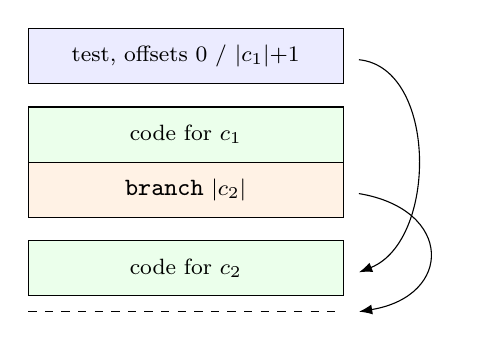
\begin{tikzpicture}[x=1mm,y=1mm,font=\footnotesize]
  \draw[fill=blue!8] (0,30) rectangle (40,37); \node at (20,33.5) {test, offsets $0$ / $|c_1|{+}1$};
  \draw[fill=green!8] (0,20) rectangle (40,27); \node at (20,23.5) {code for $c_1$};
  \draw[fill=orange!10] (0,13) rectangle (40,20); \node at (20,16.5) {\code{branch} $|c_2|$};
  \draw[fill=green!8] (0,3) rectangle (40,10); \node at (20,6.5) {code for $c_2$};
  \draw[dashed] (0,1) -- (40,1);
  \draw[-{Latex}] (42,33) .. controls (52,32) and (52,10) .. (42,6);
  \draw[-{Latex}] (42,16) .. controls (54,14) and (54,3) .. (42,1);
\end{tikzpicture}
\end{column}
\begin{column}{0.48\textwidth}
\begin{center}\textbf{while}\end{center}
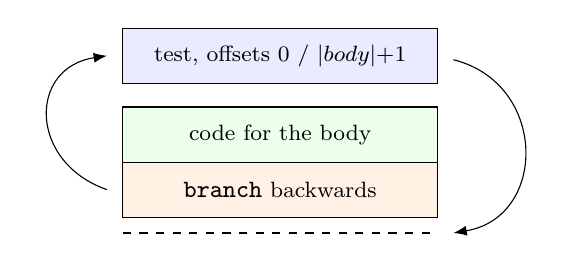
\begin{tikzpicture}[x=1mm,y=1mm,font=\footnotesize]
  \draw[fill=blue!8] (0,30) rectangle (40,37); \node at (20,33.5) {test, offsets $0$ / $|body|{+}1$};
  \draw[fill=green!8] (0,20) rectangle (40,27); \node at (20,23.5) {code for the body};
  \draw[fill=orange!10] (0,13) rectangle (40,20); \node at (20,16.5) {\code{branch} backwards};
  \draw[dashed] (0,11) -- (40,11);
  \draw[-{Latex}] (42,33) .. controls (54,30) and (54,13) .. (42,11);
  \draw[-{Latex}] (-2,16.5) .. controls (-12,20) and (-12,32) .. (-2,33.5);
\end{tikzpicture}
\end{column}
\end{columns}
\medskip

The whole program appends a \code{halt} so that it stops cleanly:
\code{compileProgram p = compileCom p ++ [.halt]}.
\end{frame}

\begin{frame}[fragile]{Examples}
\begin{lstlisting}
compileProgram (.assign "x" (.plus (.var "x") (.const 1)))
  = [.var "x", .const 1, .add, .setvar "x", .halt]

compileProgram (.while .true .skip)
  = [.branch (-1), .halt]

compileProgram (.ifthenelse (.equal (.var "x") (.const 1))
                            (.assign "x" (.const 0)) .skip)
  = [.var "x", .const 1, .beq 0 3,
     .const 0, .setvar "x", .branch 0, .halt]
\end{lstlisting}
\medskip
The last one shows a small inefficiency: \code{branch 0} does nothing.
A smart constructor fixes it --- see the exercises.
\begin{lstlisting}
def smartBranch (d : Int) : Code := if d = 0 then [] else [.branch d]
\end{lstlisting}
\end{frame}

% ===================================================================
\section{4. First correctness proofs}

\begin{frame}[fragile]{Reasoning about code fragments}
The code for a sub-expression sits \emph{inside} the code for the whole
program, at some offset.
\begin{lstlisting}
def CodeAt (C : Code) (pc : Int) (C' : Code) : Prop :=
  ∃ C₁ C₃, C = C₁ ++ C' ++ C₃ ∧ pc = codelen C₁
\end{lstlisting}
Navigation lemmas let us descend into a fragment:
\begin{lstlisting}
theorem CodeAt.head : CodeAt C pc (i :: C') → instrAt C pc = some i
theorem CodeAt.app_left  : CodeAt C pc (D₁ ++ D₂) → CodeAt C pc D₁
theorem CodeAt.app_right : CodeAt C pc (D₁ ++ D₂) →
                           CodeAt C (pc + codelen D₁) D₂
\end{lstlisting}
Every correctness statement below is relative to such a hypothesis.
\end{frame}

\begin{frame}[fragile]{4.1 Expressions}
The informal contract, now a theorem:
\begin{lstlisting}
theorem compileAexp_correct {C : Code} {s : Store} (a : aexp) :
    ∀ {pc pc' : Int} {stk : Stack},
    CodeAt C pc (compileAexp a) →
    pc' = pc + codelen (compileAexp a) →
    transitions C (pc, stk, s) (pc', aeval s a :: stk, s)
\end{lstlisting}
Read it as: starting at the beginning of the generated code with any stack,
the machine runs to the end of that code, having pushed \code{aeval s a} and
changed nothing else.
\medskip

Proof: induction on \code{a}.  For \code{plus}, chain the run of
\code{compileAexp a₁}, then that of \code{compileAexp a₂}, then one
\code{add}.
\medskip

The target program counter is a \emph{variable} \code{pc'} constrained by an
equation.  That is what lets the pieces compose without rewriting arithmetic
at every step.
\end{frame}

\begin{frame}[fragile]{4.1 Boolean expressions}
\begin{lstlisting}
theorem compileBexp_correct {C : Code} {s : Store} (b : bexp) :
    ∀ (d₁ d₀ : Int) {pc pc' : Int} {stk : Stack},
    CodeAt C pc (compileBexp b d₁ d₀) →
    pc' = pc + codelen (compileBexp b d₁ d₀)
        + (if beval s b then d₁ else d₀) →
    transitions C (pc, stk, s) (pc', stk, s)
\end{lstlisting}
The statement is the informal specification, verbatim.
\medskip

The \code{and} case is where the offsets earn their keep: after running
\code{code₁}, case on \code{beval s b₁}.  If true we are exactly at the start
of \code{code₂} and apply the induction hypothesis; if false we have already
landed at the right place and take zero further steps.
\end{frame}

\begin{frame}[fragile]{4.2 Commands, terminating case}
\begin{lstlisting}
theorem compileCom_correct_terminating {C : Code} {s c s'}
    (h : cexec s c s') :
    ∀ {pc pc' : Int} {stk : Stack},
    CodeAt C pc (compileCom c) → pc' = pc + codelen (compileCom c) →
    transitions C (pc, stk, s) (pc', stk, s')
\end{lstlisting}
Induction on the \emph{big-step derivation}, not on the command --- the
\code{while\_loop} case needs the induction hypothesis for the loop itself,
re-entered at the same \code{pc}.
\medskip

\begin{lstlisting}
theorem compileProgram_correct_terminating {s c s'} (h : cexec s c s') :
    machineTerminates (compileProgram c) s s'
\end{lstlisting}
\end{frame}

\begin{frame}{What we have, and what is missing}
\textbf{Have.}  If the source terminates in $s'$, the compiled program halts
in $s'$.
\medskip

\textbf{Missing.}  Everything about programs that do \emph{not} terminate.
\medskip

The big-step semantics simply has nothing to say: \code{while true do skip}
has no derivation, and so the theorem above is vacuous for it.  A compiler
that turned every loop into \code{halt} would satisfy it.
\medskip
\pause

To rule that out we need a semantics in which divergence is a positive
statement rather than an absence.  That means small-step.
\end{frame}

% ===================================================================
\section{6. Small-step semantics}

\begin{frame}[fragile]{6.1 Reduction semantics}
\code{red (c, s) (c', s')}: one elementary step of \code{c} in store
\code{s}, leaving residual command \code{c'}.
\begin{lstlisting}
inductive red : com × Store → com × Store → Prop where
  | assign (x a s) : red (.assign x a, s) (.skip, update x (aeval s a) s)
  | seq_done (c s) : red (.skip ;; c, s) (c, s)
  | seq_step : red (c₁, s₁) (c₂, s₂) → red (c₁ ;; c, s₁) (c₂ ;; c, s₂)
  | ifthenelse (b c₁ c₂ s) :
      red (.ifthenelse b c₁ c₂, s) ((if beval s b then c₁ else c₂), s)
  | while_done : beval s b = false → red (.while b c, s) (.skip, s)
  | while_loop : beval s b = true → red (.while b c, s) (c ;; .while b c, s)
\end{lstlisting}
Now a diverging program is one with an infinite sequence of steps --- a
positive statement.
\end{frame}

\begin{frame}[fragile]{IMP programs cannot go wrong}
\begin{lstlisting}
theorem red_progress (c : com) (s : Store) :
    c = .skip ∨ ∃ c' s', red (c, s) (c', s')

def goesWrong (c : com) (s : Store) : Prop :=
  ∃ c' s', Star red (c, s) (c', s') ∧ Irred red (c', s') ∧ c' ≠ .skip

theorem not_goesWrong (c : com) (s : Store) : ¬ goesWrong c s
\end{lstlisting}
Every non-\code{skip} command can take a step, so the only irreducible state
is \code{skip}.  Combined with compiler correctness, this is what tells us
compiled code never gets stuck either.
\end{frame}

\begin{frame}[fragile]{Big-step and small-step agree}
\begin{lstlisting}
theorem cexec_to_reds {s c s'} (h : cexec s c s') :
    Star red (c, s) (.skip, s')

theorem reds_to_cexec {s c s'} (h : Star red (c, s) (.skip, s')) :
    cexec s c s'
\end{lstlisting}
The first is a routine induction on the derivation.  The second rests on a
key lemma --- one reduction step followed by a big-step execution collapses
into a single big-step execution:
\begin{lstlisting}
theorem red_append_cexec (h : red p q) :
    ∀ {s'}, cexec q.2 q.1 s' → cexec p.2 p.1 s'
\end{lstlisting}
\end{frame}

\begin{frame}[fragile]{6.2 Transitions with continuations}
The reduction relation rebuilds a whole command at each step.  That is
awkward to relate to a machine that just moves a program counter.
\medskip

Split the configuration in two: the \textbf{sub-command under focus}, and a
\textbf{continuation} recording what remains to be done.
\begin{lstlisting}
inductive cont where
  | stop
  | seq   (c : com) (k : cont)
  | while (b : bexp) (c : com) (k : cont)
\end{lstlisting}
\code{applyCont k c} rebuilds the whole command by placing \code{c} leftmost
in the nest of sequences described by \code{k}.
\end{frame}

\begin{frame}[fragile]{Three kinds of rule}
\begin{lstlisting}
inductive step : com × cont × Store → com × cont × Store → Prop where
  -- computation
  | assign : step (.assign x a, k, s) (.skip, k, update x (aeval s a) s)
  | ifthenelse : step (.ifthenelse b c₁ c₂, k, s)
                      ((if beval s b then c₁ else c₂), k, s)
  | while_done : beval s b = false → step (.while b c, k, s) (.skip, k, s)
  -- focusing
  | seq : step (c₁ ;; c₂, k, s) (c₁, .seq c₂ k, s)
  | while_true : beval s b = true → step (.while b c, k, s) (c, .while b c k, s)
  -- resumption
  | skip_seq   : step (.skip, .seq c k, s) (c, k, s)
  | skip_while : step (.skip, .while b c k, s) (.while b c, k, s)
\end{lstlisting}
\emph{Computation} evaluates an expression and acts on the result;
\emph{focusing} descends into a sub-command; \emph{resumption} pops the
continuation when the focus is \code{skip}.
\end{frame}

\begin{frame}[fragile]{Aside: continuations extend painlessly}
Suppose we add C's \code{break}.  No existing rule changes; we add two
resumption rules:
\begin{lstlisting}
| break_seq   : step (.break, .seq c k, s)     (.break, k, s)
| break_while : step (.break, .while b c k, s) (.skip, k, s)
\end{lstlisting}
\medskip

The first says \code{break} \emph{floats up} through pending sequences,
skipping the computations they contain.  When it meets a \code{while}
continuation it has found its enclosing loop; the second discards that
continuation and turns the \code{break} into \code{skip}.
\medskip

That is the entire semantics of \code{break}.  \code{continue} is an
exercise; labelled \code{break lbl} is another.
\end{frame}

% ===================================================================
\section{7. Full compiler correctness}

\begin{frame}{Simulation diagrams}
We want: every source step is matched by machine steps, preserving a relation
$\sim$ between configurations.
\medskip
\begin{center}
\begin{tikzpicture}[x=1mm,y=1mm,font=\small]
  \node (a) at (0,20) {$c,k,s$};   \node (b) at (45,20) {$M$};
  \node (c) at (0,0)  {$c',k',s'$}; \node (d) at (45,0) {$M'$};
  \draw[dashed] (a) -- node[above,font=\scriptsize]{$\sim$} (b);
  \draw[dashed] (c) -- node[below,font=\scriptsize]{$\sim$} (d);
  \draw[-{Latex}] (a) -- (c);
  \draw[-{Latex}] (b) -- node[right,font=\scriptsize]{$+$ steps} (d);
\end{tikzpicture}
\end{center}
\medskip

Take the diagram with \emph{one or more} machine steps ($+$) and divergence
transfers immediately: infinitely many source steps give infinitely many
machine steps.
\medskip
\pause
But our compiler does not satisfy it.  Some source steps generate \emph{no}
machine transition at all --- entering a sequence, or testing a loop that
compiles to nothing.
\end{frame}

\begin{frame}{Stuttering, and how to control it}
So we allow \emph{zero} machine steps, but only finitely often in a row:
\begin{center}
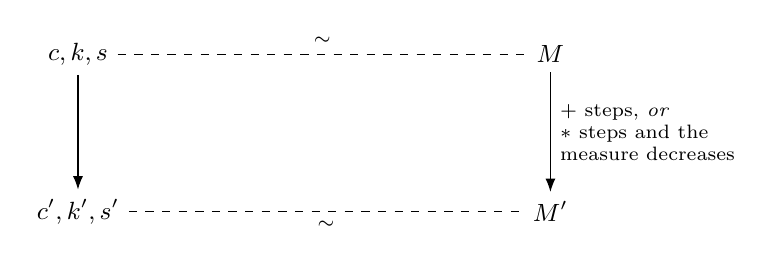
\begin{tikzpicture}[x=1mm,y=1mm,font=\small]
  \node (a) at (0,20) {$c,k,s$};   \node (b) at (60,20) {$M$};
  \node (c) at (0,0)  {$c',k',s'$}; \node (d) at (60,0) {$M'$};
  \draw[dashed] (a) -- node[above,font=\scriptsize]{$\sim$} (b);
  \draw[dashed] (c) -- node[below,font=\scriptsize]{$\sim$} (d);
  \draw[-{Latex}] (a) -- (c);
  \draw[-{Latex}] (b) -- node[right,font=\scriptsize,align=left]
     {$+$ steps, \emph{or}\\ $*$ steps and the\\ measure decreases} (d);
\end{tikzpicture}
\end{center}
\medskip

A \emph{measure} on source configurations, strictly decreasing on stuttering
steps, rules out an infinite run of them.  Without it, a compiler that
emitted \code{halt} for every loop would satisfy the diagram.
\medskip

Finding a measure is a small black art.  Here: the size of the command in
focus plus the sizes of the commands recorded in the continuation.
\end{frame}

\begin{frame}[fragile]{Relating continuations to code}
When the machine finishes the code for \code{c}, the instructions it meets
next should carry out the pending computations in \code{k}, then halt.
\begin{lstlisting}
inductive compileCont (C : Code) : cont → Int → Prop where
  | stop : instrAt C pc = some .halt → compileCont C .stop pc
  | seq  : CodeAt C pc (compileCom c) → pc' = pc + codelen (compileCom c) →
           compileCont C k pc' → compileCont C (.seq c k) pc
  | while : instrAt C pc = some (.branch d) → pc' = pc + 1 + d →
            CodeAt C pc' (compileCom (.while b c)) → ... →
            compileCont C (.while b c k) pc
  | branch : instrAt C pc = some (.branch d) → pc' = pc + 1 + d →
             compileCont C k pc' → compileCont C k pc
\end{lstlisting}
The last rule matters: a continuation may sit behind a \emph{chain of
unconditional jumps}.
\end{frame}

\begin{frame}[fragile]{The matching relation and the measure}
\begin{lstlisting}
inductive matchConfig (C : Code) : com × cont × Store → Config → Prop where
  | intro : CodeAt C pc (compileCom c) →
            compileCont C k (pc + codelen (compileCom c)) →
            matchConfig C (c, k, st) (pc, [], st)
\end{lstlisting}
Same store; empty machine stack; code for \code{c} at \code{pc}; code
carrying out \code{k} after it.
\begin{lstlisting}
def comSize : com → Nat
  | .skip | .assign _ _ => 1
  | .seq c₁ c₂ | .ifthenelse _ c₁ c₂ => comSize c₁ + comSize c₂ + 1
  | .while _ c₁ => comSize c₁ + 1

def measure : com × cont × Store → Nat
  | (c, k, _) => comSize c + contSize k
\end{lstlisting}
\end{frame}

\begin{frame}[fragile]{The simulation theorem}
\begin{lstlisting}
theorem simulation_step {C : Code} {ic₁ ic₂ : com × cont × Store}
    {mc₁ : Config}
    (hstep : step ic₁ ic₂) (hmatch : matchConfig C ic₁ mc₁) :
    ∃ mc₂, (Plus (transition C) mc₁ mc₂
            ∨ (transitions C mc₁ mc₂ ∧ measure ic₂ < measure ic₁))
      ∧ matchConfig C ic₂ mc₂
\end{lstlisting}
Seven cases, one per rule of \code{step}.
\medskip

\begin{itemize}
\item \code{assign} and \code{skip\_while} take the $+$ branch.
\item \code{seq}, \code{ifthenelse}, \code{while\_done}, \code{while\_true},
      \code{skip\_seq} take the $*$-with-measure branch.
\end{itemize}
\medskip

This is the hard work of the development.  Everything below is a corollary.
\end{frame}

\begin{frame}[fragile]{Corollary 1: termination, again}
\begin{lstlisting}
theorem simulation_steps (h : Star step ic₁ ic₂) :
    ∀ {mc₁}, matchConfig C ic₁ mc₁ →
    ∃ mc₂, transitions C mc₁ mc₂ ∧ matchConfig C ic₂ mc₂

theorem compileProgram_correct_terminating_2 {c : com} {s s' : Store}
    (h : Star step (c, .stop, s) (.skip, .stop, s')) :
    machineTerminates (compileProgram c) s s'
\end{lstlisting}
A second proof of the \S4 result, now from the continuation semantics.
\end{frame}

\begin{frame}[fragile]{Corollary 2: divergence}
\begin{lstlisting}
theorem compileProgram_correct_diverging {c : com} {s : Store}
    (h : Infseq step (c, .stop, s)) : machineDiverges (compileProgram c) s
\end{lstlisting}
The bridge is a lemma saying that from a diverging source configuration the
machine can always make \emph{at least one} transition into a configuration
that again matches a diverging source configuration:
\begin{lstlisting}
theorem simulation_infseq_inv : ∀ (n : Nat) {ic₁ mc₁},
    Infseq step ic₁ → matchConfig C ic₁ mc₁ → measure ic₁ < n →
    ∃ ic₂ mc₂, Infseq step ic₂ ∧ Plus (transition C) mc₁ mc₂
             ∧ matchConfig C ic₂ mc₂
\end{lstlisting}
The bound \code{n} on the measure turns this into an ordinary induction:
consecutive stuttering steps must run out.
\end{frame}

\begin{frame}[fragile]{Interlude: divergence in Lean}
Coq defines divergence with \code{CoInductive} --- a \emph{greatest}
fixpoint.  Lean 4 has no coinductive types, so we take the greatest fixpoint
by hand.  For $\Phi(X) = \{a \mid \exists b,\ R\,a\,b \wedge b \in X\}$,
Knaster--Tarski gives
\[ \nu\Phi \;=\; \bigcup\,\{\,X \mid X \subseteq \Phi(X)\,\}. \]
Written out, that is the definition:
\begin{lstlisting}
def Infseq (R : A → A → Prop) (a : A) : Prop :=
  ∃ X : A → Prop, X a ∧ ∀ x, X x → ∃ y, R x y ∧ X y
\end{lstlisting}
\code{X} is an \emph{invariant}: from every member you can step and stay
inside.  So you can never get stuck.
\medskip

An \code{inductive} definition would be the \emph{least} fixpoint --- which,
having no base case, is empty.
\end{frame}

\begin{frame}[fragile]{The coinduction principle is the definition}
\begin{lstlisting}
theorem Infseq.coinduction {X : A → Prop}
    (hX : ∀ x, X x → ∃ y, R x y ∧ X y) (ha : X a) : Infseq R a :=
  ⟨X, ha, hX⟩
\end{lstlisting}
In Coq this needs \code{cofix} and a guardedness check.  Here it is just
repackaging.
\medskip

The constructor and destructor are recovered as lemmas, so
$\mathrm{Infseq} = \Phi(\mathrm{Infseq})$ really is a fixpoint.
\medskip

And the payoff, in the divergence proof: the invariant supplied is
\begin{center}
\emph{``this machine configuration matches some diverging source
configuration''}
\end{center}
--- that is, the invariant \emph{is} the simulation relation, named and
visible.
\end{frame}

% ===================================================================
\section{8. Constant propagation}

\begin{frame}[fragile]{8.1 Smart constructors}
Build the simplified expression instead of building then simplifying:
\begin{lstlisting}
def mkPlusConst (a : aexp) (n : Int) : aexp :=
  if n = 0 then a else
    match a with
    | .const m => .const (m + n)
    | .plus a (.const m) => .plus a (.const (m + n))
    | _ => .plus a (.const n)
\end{lstlisting}
\code{mkPlus} uses associativity and commutativity to expose the pattern
``expression plus constant''; \code{mkMinus} normalises ``expression minus
constant'' into ``expression plus the opposite constant''.
\begin{lstlisting}
theorem mkPlus_sound (s : Store) (a₁ a₂ : aexp) :
    aeval s (mkPlus a₁ a₂) = aeval s a₁ + aeval s a₂
\end{lstlisting}
Commands benefit too: \code{mkIfthenelse} and \code{mkWhile} take known
conditions into account.
\end{frame}

\begin{frame}[fragile]{8.2 Abstract stores}
An \emph{abstract store} records what the analysis knows.  If it maps
\code{x} to \code{n}, then \code{x} certainly holds \code{n} at run time; if
it maps \code{x} to nothing, \code{x} may hold anything.
\medskip

So \emph{less information} means \emph{larger}, and the top element is the
empty map.
\begin{lstlisting}
def Matches (s : Store) (S : AStore) : Prop :=
  ∀ x n, S.find x = some n → s x = n

def Le (S₁ S₂ : AStore) : Prop :=
  ∀ x n, S₂.find x = some n → S₁.find x = some n
\end{lstlisting}
\code{Matches} is the concretisation relation --- a bit like ``a term has a
type''.  The join keeps only the facts two stores agree on.
\medskip

{\small (Coq uses \code{FMaps}; Lean's core has no finite maps, so these are
association lists.)}
\end{frame}

\begin{frame}[fragile]{Abstract evaluation}
\begin{lstlisting}
def Aeval (S : AStore) : aexp → Option Int
  | .const n => some n
  | .var x   => S.find x
  | .plus a₁ a₂ => match Aeval S a₁, Aeval S a₂ with
      | some n₁, some n₂ => some (n₁ + n₂)
      | _, _ => none
  | ...
\end{lstlisting}
\code{some v} means ``the value is certainly \code{v}''; \code{none} means
``unknown''.  Soundness relates the two worlds:
\begin{lstlisting}
theorem Aeval_sound (hm : Matches s S) :
    ∀ (a : aexp) {n : Int}, Aeval S a = some n → aeval s a = n
\end{lstlisting}
\end{frame}

\begin{frame}[fragile]{The analysis}
\begin{lstlisting}
def Cexec (S : AStore) (c : com) : AStore :=
  match c with
  | .skip => S
  | .assign x a => AStore.update x (Aeval S a) S
  | .seq c₁ c₂ => Cexec (Cexec S c₁) c₂
  | .ifthenelse b c₁ c₂ => match Beval S b with
      | some true  => Cexec S c₁
      | some false => Cexec S c₂
      | none => AStore.join (Cexec S c₁) (Cexec S c₂)
  | .while _ c₁ => fixpoint (fun X => AStore.join S (Cexec X c₁)) S
\end{lstlisting}
Loops need a fixpoint --- executing the loop in the abstract until the
abstract state stops changing.  For now, the engineer's answer: iterate
twenty times, and fall back on \code{top} (know nothing).  Imprecise, but
sound, and \S9 will do better.
\end{frame}

\begin{frame}[fragile]{Soundness of the analysis}
\begin{lstlisting}
theorem fixpoint_sound (F : AStore → AStore) (initS : AStore) :
    Le (F (fixpoint F initS)) (fixpoint F initS)

theorem Cexec_sound : ∀ (c : com) {s₁ s₂ : Store} {S₁ : AStore},
    cexec s₁ c s₂ → Matches s₁ S₁ → Matches s₂ (Cexec S₁ c)
\end{lstlisting}
The \emph{only} property of \code{fixpoint} used is that it returns a
post-fixpoint.  Precision is not needed for soundness.
\medskip

The \code{while} case needs an unusual induction: structural on the command,
plus an inner induction on the iterations actually performed.  That pattern
mirrors the structure of \code{Cexec} itself.
\end{frame}

\begin{frame}[fragile]{8.3 The optimisation}
\begin{lstlisting}
def cpCom (S : AStore) (c : com) : com :=
  match c with
  | .skip => .skip
  | .assign x a => .assign x (cpAexp S a)
  | .seq c₁ c₂ => .seq (cpCom S c₁) (cpCom (Cexec S c₁) c₂)
  | .ifthenelse b c₁ c₂ =>
      mkIfthenelse (cpBexp S b) (cpCom S c₁) (cpCom S c₂)
  | .while b c₁ =>
      let sfix := Cexec S (.while b c₁)
      mkWhile (cpBexp sfix b) (cpCom sfix c₁)
\end{lstlisting}
\code{S} is what is known \emph{before} \code{c}, so it must be threaded
exactly as the analysis threads it.
\begin{lstlisting}
theorem cpCom_correct_terminating : ∀ (c : com) {s₁ s₂ S₁},
    cexec s₁ c s₂ → Matches s₁ S₁ → cexec s₁ (cpCom S₁ c) s₂
\end{lstlisting}
\end{frame}

% ===================================================================
\section{9. More about fixpoints}

\begin{frame}{9.1 From Knaster--Tarski to computation}
Let $F$ be monotone on a set with a decidable equality, a transitive order,
and a \textbf{well-founded strict order} --- every strictly ascending chain
is finite.
\medskip

\textbf{Knaster--Tarski.}  $F$ has a fixpoint.
\medskip

The proof is already an algorithm: start from a pre-fixpoint $x \le F(x)$;
either $x = F(x)$ and we are done, or $F(x)$ is strictly above $x$ and is
itself a pre-fixpoint, so recurse.  Well-foundedness makes the recursion
terminate.
\medskip
\pause

But an existence proof $\exists x,\ x = F(x)$ gives no way to \emph{compute}
$x$.  Pattern-matching on it to extract the witness is not allowed.
\end{frame}

\begin{frame}[fragile]{Producing the value, not just its existence}
Return a \emph{subtype} instead --- the value packaged with its
specification:
\begin{lstlisting}
def iterate (Fmon : ∀ x y, L.le x y → L.le (F x) (F y)) :
    ∀ (x : A), L.le x (F x) → (∀ z, L.le (F z) z → L.le x z) →
      { y : A // L.eq y (F y) ∧ ∀ z, L.le (F z) z → L.le y z } :=
  L.gt_wf.fix fun x ih hpre hsmall =>
    match hb : L.beq x (F x) with
    | true  => ⟨x, L.beq_eq hb, hsmall⟩
    | false => ih (F x) ⟨hpre, L.beq_neq hb⟩ (Fmon _ _ hpre)
                 (fun z hz => L.le_trans (Fmon _ _ (hsmall z hz)) hz)
\end{lstlisting}
It carries a pre-fixpoint \emph{and} a proof that it is below every
post-fixpoint, and returns a fixpoint that is still below every
post-fixpoint --- the \emph{least} one.
\medskip

Coq writes this with \code{Program Fixpoint}, leaving holes for the proofs.
Lean uses \code{WellFounded.fix} directly.
\end{frame}

\begin{frame}[fragile]{9.2 Application: the hard part}
To use this for abstract stores we must show the strict order is well
founded.  Measure a store by the number of \emph{distinct} variables it
pins down:
\begin{lstlisting}
theorem Le_card {S T : AStore} (h : Le T S) :
    card S ≤ card T ∧ (card S = card T → AEq T S)

theorem Gt_wf : WellFounded (fun S S' => Le S' S ∧ ¬ AEq S' S)
\end{lstlisting}
Going strictly up in the order means losing at least one fact, so the
measure strictly decreases --- and \code{Nat} is well founded.
\medskip

{\small Coq reasons about the \emph{cardinal} of a finite map.  With
association lists we reason about the length of the deduplicated key list,
which needs two combinatorial lemmas about duplicate-free lists.}
\end{frame}

\begin{frame}[fragile]{9.2 The second obstacle: no bottom}
Abstract stores have no smallest element, so we cannot iterate from one.
\medskip

But for the functions we care about there \emph{is} a natural starting point:
the store \code{init} describing what is known on entry to the loop.  Iterate
$X \mapsto \mathit{init} \sqcup F(X)$, which is above \code{init} by
construction.
\begin{lstlisting}
def fixpointJoin (init : AStore) (F : AStore → AStore) (hF : Increasing F)
    : AStore

theorem fixpointJoin_sound :
    Le init (fixpointJoin init F hF)
  ∧ Le (F (fixpointJoin init F hF)) (fixpointJoin init F hF)

theorem fixpointJoin_smallest (S : AStore) :
    Le (AStore.join init (F S)) S → Le (fixpointJoin init F hF) S
\end{lstlisting}
\end{frame}

\begin{frame}[fragile]{Definition and proof, simultaneously}
Now try to rebuild the analyser using \code{fixpointJoin}\ldots{} and it does
not typecheck: \emph{only increasing functions have fixpoints}, and the loop
case needs to know the body is increasing.
\medskip

So the function must return its own proof:
\begin{lstlisting}
def CexecM : com → { F : AStore → AStore // Increasing F }
  | .skip => ⟨id, fun _ _ h => h⟩
  | .assign x a => ⟨fun S => AStore.update x (Aeval S a) S,
                    fun _ _ h => update_increasing x a h⟩
  | .seq c₁ c₂ => ⟨fun S => (CexecM c₂).1 ((CexecM c₁).1 S), ...⟩
  | .while _ c₁ => ⟨fun S => fixpointJoin S (CexecM c₁).1 (CexecM c₁).2,
                    fun _ _ h => fixpointJoin_increasing _ _ h⟩
\end{lstlisting}
Definition and monotonicity proof are constructed in one go --- there is no
way to separate them.
\end{frame}

% ===================================================================
\section{10. Liveness and dead code elimination}

\begin{frame}[fragile]{10.1 Liveness analysis}
A variable is \textbf{live} at a program point if some later instruction may
read it before it is overwritten.  An assignment to a variable that is not
live is \emph{dead}.
\medskip

This is a \textbf{backward} analysis --- contrast constant propagation:
\code{live c L} is the set live \emph{before} \code{c}, given that \code{L}
is live \emph{after} it.
\begin{lstlisting}
def live (c : com) (L : IdentSet) : IdentSet :=
  match c with
  | .skip => L
  | .assign x a => if x ∈ L then remove x L ++ fvAexp a else L
  | .seq c₁ c₂ => live c₁ (live c₂ L)
  | .ifthenelse b c₁ c₂ => fvBexp b ++ (live c₁ L ++ live c₂ L)
  | .while b c => fixpoint (fun x => (fvBexp b ++ L) ++ live c x)
                           (fvCom (.while b c) ++ L)
\end{lstlisting}
Note the assignment case: if \code{x} is live after, it stops being live
before, and everything \code{a} reads becomes live.
\end{frame}

\begin{frame}[fragile]{10.2 The optimisation}
\begin{lstlisting}
def dce (c : com) (L : IdentSet) : com :=
  match c with
  | .skip => .skip
  | .assign x a => if x ∈ L then .assign x a else .skip
  | .seq c₁ c₂ => .seq (dce c₁ (live c₂ L)) (dce c₂ L)
  | .ifthenelse b c₁ c₂ => .ifthenelse b (dce c₁ L) (dce c₂ L)
  | .while b c => .while b (dce c (live (.while b c) L))
\end{lstlisting}
On Euclidean division, keeping only \code{"r"} live at the end:
\begin{lstlisting}
r := a;              ===>   r := a;
q := 0;                     skip;
while b <= r do             while b <= r do
  r := r - b;                 r := r - b;
  q := q + 1                  skip
\end{lstlisting}
Keeping \code{"q"} live instead, nothing can be removed.
\end{frame}

\begin{frame}[fragile]{10.3 Correctness}
The optimised program runs in a store that may \emph{differ} from the
original on dead variables --- that is the whole point.  So the invariant is
agreement on the live ones.
\begin{lstlisting}
def agree (L : IdentSet) (s₁ s₂ : Store) : Prop :=
  ∀ x, x ∈ L → s₁ x = s₂ x
\end{lstlisting}
\begin{center}
\begin{tikzpicture}[x=1mm,y=1mm,font=\small]
  \node (a) at (0,18) {$c,s$};   \node (b) at (55,18) {$\mathrm{dce}\ c\ L,\ s_1$};
  \node (c) at (0,0)  {$s'$};    \node (d) at (55,0) {$s_1'$};
  \draw[dashed] (a) -- node[above,font=\scriptsize]{$\mathrm{agree}\ (\mathrm{live}\ c\ L)$} (b);
  \draw[dashed] (c) -- node[below,font=\scriptsize]{$\mathrm{agree}\ L$} (d);
  \draw[-{Latex}] (a) -- (c); \draw[-{Latex}] (b) -- (d);
\end{tikzpicture}
\end{center}
\begin{lstlisting}
theorem dce_correct_terminating {s c s'} (h : cexec s c s') :
    ∀ (L : IdentSet) (s₁ : Store), agree (live c L) s s₁ →
    ∃ s₁', cexec s₁ (dce c L) s₁' ∧ agree L s' s₁'
\end{lstlisting}
\end{frame}

% ===================================================================
\section{Closing}

\begin{frame}{What we proved}
\begin{itemize}\setlength{\itemsep}{4pt}
\item A compiler from IMP to a stack machine, with semantic preservation for
      \emph{terminating and diverging} programs.
\item Constant propagation: a forward dataflow analysis, its soundness, and
      the optimisation built on it.
\item Dead code elimination: a backward analysis and its optimisation.
\item The fixpoint theory that makes the analyses precise, with a
      terminating algorithm.
\end{itemize}
\medskip

All machine-checked, with no \code{sorry}, in about 3\,000 lines of Lean~4
and no dependencies beyond the core library.
\end{frame}

\begin{frame}{What scales, and what does not}
The \emph{methods} scale: this is how CompCert --- a verified C compiler,
with a dozen intermediate languages and many more optimisations --- is
built.
\medskip

What gets harder:
\begin{itemize}
\item real languages have memory, pointers, function calls, undefined
      behaviour;
\item real machines have registers and a finite number of them;
\item simulation diagrams compose, but the invariants get big.
\end{itemize}
\medskip

What stays the same: semantics first, then a simulation relation, then a
measure to control stuttering.
\end{frame}

\begin{frame}{Further reading}
\begin{itemize}\setlength{\itemsep}{4pt}
\item Xavier Leroy. \emph{Formal verification of a realistic compiler}.
      Comm.\ ACM 52(7):107--115, 2009.
\item Xavier Leroy. \emph{A formally verified compiler back-end}.
\item Benjamin Pierce et al. \emph{Software Foundations}.
\item Yves Bertot. \emph{Structural abstract interpretation, a formal study
      using Coq}.
\end{itemize}
\vfill
{\small Original course and Coq sources:
\texttt{https://xavierleroy.org/courses/EUTypes-2019/}}
\end{frame}

\end{document}
